\documentclass{article}

\usepackage[utf8]{inputenc}
\usepackage{setspace}
\usepackage[
	a4paper,
	total={17cm,25cm},
	top=3cm, left=2cm,
	includefoot
	]{geometry}
\usepackage[
	english,
	czech
	]{babel}
\usepackage[autostyle]{csquotes}
\usepackage{caption}
\usepackage{graphicx}
\graphicspath{{./assets/}}

\title{Správa Office 365}
\author{Petr Maronek}
\date{5.11.2022}

% 	Vysvětlivky
%	\section* hvězdička znamená, že má LaTeX odebrat číslování

\begin{document}
    \begin{sloppypar}
	\begin{spacing}{1.15}
		\rmfamily
		\maketitle
		\begin{center}
			\textbf{Vysoká škola finanční a správní}\linebreak
			Projektování Informačních Systémů 1\linebreak
			Zimní semestr 2022\linebreak
			Vedoucí práce: \textbf{Ing. Václav Řezníček, Ph.D.}
		\end{center}
		\pagebreak
			
		\section*{Abstrakt}
		Správa Officu 365, konkrétně SharePointu Online a Microsoft Teams, je pro velké 
        firmy čím dál náročnější. Má aplikace, kterou tato práce popisuje a implementuje, 
        se tuto problematiku pokouší přímo vyřešit a celou správu tak učinit přístupnější 
        pro administraci a případnou rozšiřitelnost. Spolu s modelem správy, který musí 
        zajistit korporátní zásady pro uchování dat, je také zásadní implementace v cloudovém 
        prostředí Microsoft Azure. Celý model zohledňuje požadavky na retenci dat, bezpečnost 
        z hlediska přístupů a datové hygieny.

		\section*{Klíčová slova}
		Office365, Microsoft, proces, automatizace, korporace, cloud
		\pagebreak
		    
		\section*{Úvod}
	    Office 365 je rozsáhlý ekosystém byznysových aplikací, které pracovníkům
        v mnoha ohledech usnadňují každodenní pracovní povinnosti. Jedná se o 
        nejrozšířenější kancelářský software na světě a mnoho velkých 
        nadnárodních korporací jej používá v mnoha aspektech své činnosti. 
        Tato činnost však může být svázána místními předpisy nebo regulací 
        podnikání v určité oblasti, jako například farmacie, energetika nebo 
        potravinářství. Z této podstaty ovšem vyplývá, že se tento software musí
        řídit zásadami a politikami jednotlivých firem, aby splňoval různá 
        omezení nebo dokonce blokovat některé ze svých funkcí. V této práci se 
        zaměřím hlavně na SharePoint Online a Microsoft Teams, které jsou v celém 
        ekosystému Office 365 nejvíce používané, zejména jako úložiště dokumentů 
        a centrum sdílení napříč jednotlivými divizemi firmy. Právě životní 
        cyklus dokumentů je základní linií v každé firemní politice, která 
        podléhá místním regulím nebo externím auditům.

        Jak nejlépe poskytnout uživatelům přístup k těmto technologiím a zároveň 
        zajistit shodu s firemními a státními předpisy? Také nemůžeme spoléhat na 
        uživatele, že budou aktivně dodržovat všechna pravidla a nařízení, která 
        dané úložiště musí splňovat. V neposlední řadě musí být celé řešení do 
        jisté míry automatizované, aby administrátorský tým Office 365 nebyl 
        zavalen desítkami až stovkami požadavků denně na vytvoření SharePointu 
        nebo Teams.
        
        \section*{Současný stav}
        V této sekci projdu celé stávající řešení, jeho výhody a naopak nevýhody
        z hlediska nákladů na provoz, administrace a uživatelské přístupnosti.
        Nejprve nastíním pohled na celý systém a čemu slouží a poté provedu SWOT
        analýzu, podle které identifikuji potencionální slabiny a možnosti ke
        zlepšní.

        Systém má za primární úkol poskytnout uživatelům jednoduchou správu nad
        svými virtuálními prostory v rámci Office 365, zejména SharePoint a MS
        Teams. Obě tyto aplikace budu pro účely této práce nazývat jako
        "pracovní prostory". Systém ve svém rámci řídí důležité procesy, které 
        jsou v souladu s certifikacemi informačních technologií a navíc splňuje 
        politiky nastavené svou společností. Procesy v systému jsou například 
        vytvoření pracovního prostoru, smazání pracovního prostoru, automatické
        notifikace o expiraci pracovních prostorů nebo cybějících metadatech a
        nebo zažádání o speciální funkce v rámci těchto prostorů. Systém také
        automaticky nastavuje spoustu vlastností pro tyto prostory jako jsou
        přístupová práva, firemní branding nebo nasazení povinných firemních
        aplikací. Je tedy zřejmé, že systém není vytvořen pouze pro uživatele,
        ale také zajišťuje shodu s firemními politikami.

        Z technického hlediska je celý systém v současnoti nasazen v cloudovém 
        prostředí poskytovaném Microsoftem Azure. Nicméně celé řešení je stále 
        koncipováno do podoby, jak bylo původně vytvořené pro hostování na 
        vlastních serverch spolu s technologiemi té doby. celé řešení je v 
        současné době již přes 5 let staré a i když stále funguje podle firemních 
        požadavků, může v blízké budoucnosti dojít k jeho častým poruchám. to by
        znamenalo pro firmu v krajním případě i nemalé ztráty. A právě proto se 
        nyní pokusím zjistit, jak tomuto scénáři předejít.

        \subsection*{SWOT Analýza}
        Nejprve se zaměřím na \textbf{silné stránky} současného řešení. Protože
        je systém z části poskytovaný softwarovým dodavatelem třetí strany
        (hlavně z důvodu uživatelského rozhraní), je z podstaty velice stabilní a
        dostupnost se pohybuje v horních 99\%. Díky tomu mají uživatelé důvěru v
        systém samotný a zbytečně negenerují emaily směrem k podpoře. Pro
        uživatele je zde také samotné prostředí, ve kterém se pohybují.
        Microsoft sice poskytuje grafické prostředí pro vytváření amíněných
        prostorů, nicméně se jedná o prostředí, které není příliš intuitivní a 
        z administrátorského hlediska příliš strohé na jakkoukoliv
        rozšiřitelnost. Proto se firma před pěti lety rozhodla využít software
        třetí strany, aby poskytla uživatelům portál pro všechny své požadavky.
        Další silnou stránkou jsou nízké nároky na správu a to je zejména pro 
        administrátory velkou devízou. Tím, že se nemusí stále starat o chod
        systému, mohou svou práci přesunout jinam, kde jsou více potřeba. Systém
        stále vyžaduje jistou úroveň administrace, je nicméně znatelně ponížená
        oproti jiným řešením. Neposledním pozitivem současné řešení je také
        softwarová podpora, která je poskytována právě dodavatelskou
        společností. Ochota a rychlost řešení problémů je v tomto případě
        vitální a proto ji zařazuji mezi sné stránky.

        Nyní \textbf{slabé stránky}. Protože je software dodáván, není jednduché
        ho jakkoliv přizpůsobit požadavkům ať už administrátorů, tak firmy. Celý
        software je dodáván "AS-IS" a poskytuje minimální možnosti dodatečné
        konfigurace. 

        \begin{center}
            \label{SWOT Analýza}
            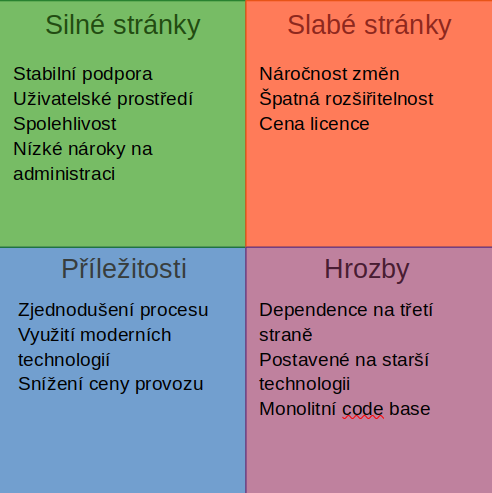
\includegraphics[scale=0.5]{221129-PIS1-SWOT.png}
            \captionof{figure}{SWOT Analýza}
        \end{center}

        \section*{Návrh budoucího stavu}
        
        \section*{Požadavky na systém}
        
        \section*{Implementace a omezení}
		
        	
	\end{spacing}
    \end{sloppypar}
\end{document}

